\documentclass[10pt]{article}
\usepackage{geometry}                % See geometry.pdf to learn the layout options. There are lots.
\geometry{a4paper
}                   % ... or a4paper or a5paper or ... 
\usepackage[parfill]{parskip}    % Activate to begin paragraphs with an empty line rather than an indent

%%%%%%%%%%%%%%%%%%%%
\newcommand{\hide}[1]{}

\usepackage{natbib}
\usepackage{xcolor}
\usepackage{url}
\usepackage{hyperref}
\usepackage{mathtools}
\usepackage{array}
\usepackage{multirow}
\usepackage{graphicx}
\usepackage{subcaption}
\usepackage{mwe}
\usepackage{float}
\usepackage{tikz}
\usepackage{booktabs}

\usepackage[nomarkers,figuresonly]{endfloat}
\usepackage[toc,page]{appendix}
\usepackage{url}

\hide{
\usepackage{amscd}
\usepackage{amsfonts}
\usepackage{amsmath}
\usepackage{amssymb}
\usepackage{amsthm}
\usepackage{cases}		 
\usepackage{cutwin}
\usepackage{enumerate}
\usepackage{epstopdf}
\usepackage{graphicx}
\usepackage{ifthen}
\usepackage{lipsum}
\usepackage{mathrsfs}	
\usepackage{multimedia}
\usepackage{wrapfig}
}

	 
%\input{/usr/local/LATEX/Lee_newcommands.tex}
\newcommand{\itemlist}[1]{\begin{itemize}#1\end{itemize}}
\newcommand{\enumlist}[1]{\begin{enumerate}#1\end{enumerate}}
\newcommand{\desclist}[1]{\begin{description}#1\end{description}}

\newcommand{\Answer}[1]{\begin{quote}{\color{blue}#1}\end{quote}}
\newcommand{\AND}{\wedge}
\newcommand{\OR}{\vee}
\newcommand{\ra}{\rightarrow}
\newcommand{\lra}{\leftrightarrow}

\newcommand\MyBox[1]{%
  \fbox{\parbox[c][.7cm][c]{.7cm}{\centering #1}}%
}
\newcommand\MyVBox[1]{%
  \parbox[c][.7cm][c]{1cm}{\centering\bfseries #1}%
}
\newcommand\MyHBox[2][\dimexpr.7cm+2\fboxsep\relax]{%
  \parbox[c][1cm][c]{#1}{\centering\bfseries #2}%
}
\usepackage{etoolbox}
\newcommand\MyTBox[2]{%
  \MyVBox{#1}
  \renewcommand*\do[1]{\MyBox{##1}\hspace*{-\fboxrule}}
  \docsvlist{#2}
  \par\vspace{-\fboxrule}
}

\title {CS36110 Machine Learning Assignment}


\date{}                                           % Activate to display a given date or no date

\begin{document}
\maketitle

I ended up with a word count of 1,656. This is excluding the figure captions, titles and appendix.

\section*{Task 1}

\subsection*{Part A}
The first algorithm I used was the J48 Decision Tree classifier this is an implementation of the ID3 algorithm with Rule Post-Pruning. ID3 grows a decision tree recursively where at each node it selects the feature with the highest information gain that best classifies the training data it was given, when the tree is grown Rule Post-Pruning (RPP) is then run over the entire tree. RPP converts each path through the tree to a rule and then independently evaluates each rule to see if it affects the validation accuracy of the tree and if it doesn't then it is pruned out. J48 mitigates overfiting because it uses RPP this helps the algorithm make a decision tree that more accurately fits the patterns in the data instead of fitting to the data itself.

The second classifier I used was Naive Bayes and it works by calculating the probabilities of events occurring within the data set it does this using Bayes Theorem and works be relating the Posterior Probability $(P(A \mid B))$ with the prior probability of the hypothesis $(P(A))$ and the conditional probability of the data under the hypothesis $(P(B \mid A))$. To classify a new piece of data you work out the probability for each decision class using the training data and the class with the highest probability is the one that you assign that data to. Naive Bayes doesn't go through a long training sequence so this makes it very fast to both classify new pieces of information and update the weights when new training data comes in.

An advantage J48 has over Naive Bayes is that Naive Bayes assumes that all the data is independent which isn't true and in real life applications this can cause the trained model to have low accuracy.

\subsection*{Part B}
In many cases overall classification accuracy is not a good indicator of a models performance especially when class data is imbalanced which is the case here because there are more class E absences then any other. So we need to look at class specific performance. One of these is precision and this along with all the other metrics for this question is shown in table \ref{tab:measuretable}. We can see that generally the model has a much higher precision score when predicting class E absences, this is could be because of the larger amount of training data for class E.

When there is a high precision score but a low recall score it means that the classifier is accurate but struggles to classify difficult instances. This is happening for class C in Naive Bayes because there is a precision score of 0.671 and a recall score of 0.292.

Class E has significantly better classifier performance than other classes this is probably due to having a higher amount of training data for class E, in every measure on both classifiers E has the highest score.

F-Measure is useful to compare because it takes into account both recall and precision and tells you how robust and precise your classifier is, the F-Measure also shows the low performance of Naive Bayes in classifying absence class C. When training a classifier there is a trade off between precision and recall because if you see an increase in precision then you would normally see a drop off in recall and vice versa\cite{minaee_2019}, it's good to know what you would like for your specific circumstances. 

\begin{table}[]
\begin{tabular}{|l|l|l|l|l|l|l|}
\hline
\begin{tabular}[c]{@{}l@{}}Absence\\  Class\end{tabular}  & \begin{tabular}[c]{@{}l@{}}NB \\ Precision\end{tabular} & \begin{tabular}[c]{@{}l@{}}J48 \\ Precision\end{tabular} & \begin{tabular}[c]{@{}l@{}}NB \\ Recall\end{tabular} & \begin{tabular}[c]{@{}l@{}}J48 \\ Recall\end{tabular} & NB F-Measure & J48 F-Measure \\ \hline
A             & 0.457        & 0.704         & 0.592     & 0.704      & 0.516        & 0.704         \\ \hline
B             & 0.467        & 0.652         & 0.616     & 0.648      & 0.531        & 0.650         \\ \hline
C             & 0.671        & 0.724         & 0.292     & 0.655      & 0.407        & 0.688         \\ \hline
E             & 0.711        & 0.777         & 0.707     & 0.843      & 0.709        & 0.809         \\ \hline
\end{tabular}
\caption{ A  table  showing  the  Precision, Recall and F-Measure for Naive Bayes (NB) and J48}
\label{tab:measuretable}
\end{table}

Figures \ref{fig:j48 confusion matrix} and \ref{fig:nb confusion matrix} below show the confusion matrices for the J48 classifier and the Naive Bayes classifier, from these matrices you can see how well the classifiers perform. You can clearly see how much better the J48 classifier is compared to Naive Bayes, if you look at the leading diagonal for J48 then you can see how much better it is. If you look at class C for Naive Bayes this inaccuracy really shows because only 49 instances where correctly classified with the majority being incorrectly classified as B this is an accuracy of only 29\%.

%J48 confusion Matrix
\begin{figure*}
    \centering
    {
    \offinterlineskip
    \hspace*{1cm}\MyHBox{A}\MyHBox{B}\MyHBox{C}
    \MyHBox{E}\par
    
    \MyTBox{A}{107, 20, 11, 14}
    \MyTBox{B}{23, 103, 20, 13}
    \MyTBox{C}{13, 24, 110,  21}
    \MyTBox{E}{9,  11,  11, 167}
    }
    \caption{The confusion matrix for the J48 decision tree classifier.}
    \label{fig:j48 confusion matrix}
\end{figure*}

%NB confusion Matrix
\begin{figure*}
    \centering
    {
    \offinterlineskip
    \hspace*{1cm}\MyHBox{A}\MyHBox{B}\MyHBox{C}
    \MyHBox{E}\par
    
    \MyTBox{A}{90,  27,  10,  25}
    \MyTBox{B}{40,  98,  10,  11}
    \MyTBox{C}{40,  58,  49,  21}
    \MyTBox{E}{27,  27,   4, 140}
    }
    \caption{The confusion matrix for the Naive Bayes classifier.}
    \label{fig:nb confusion matrix}
\end{figure*}

The Kappa statistic compares an observed accuracy with an expected accuracy and is useful in evaluating classifiers because it takes into account the random chance this makes it generally less misleading than accuracy. The Kappa statistic for Naive Bayes is 0.4091 and for J48 it is 0.6239, There is not a standardized interpretation of this statistic but Landis and Koch\cite{landiskochkappa} consider 0-0.20 as slight, 0.21-0.40 as fair, 0.41-0.60 as moderate, 0.61-0.80 as substantial, and 0.81-1 as almost perfect. Under this Naive Bayes would be classified as moderate and J48 as substantial. 

The dataset seems to contains lots of instance that have the same  conditional feature values but a different decision feature. This could be leading to poor performance and may be solved by getting more data points so that you can differentiate different absences better.

I talk about Receive Operator Characteristics in appendix \ref{appendix:roc}.

\begin{figure*}
    \centering
    \begin{subfigure}[b]{0.475\textwidth}
        \centering
        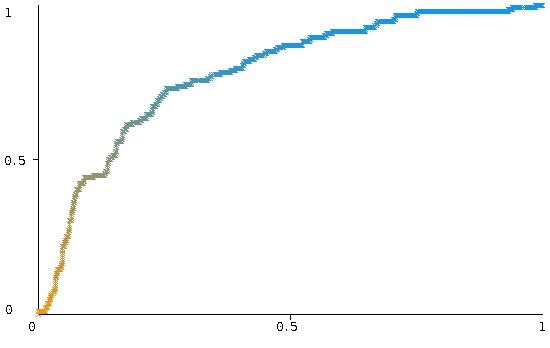
\includegraphics[width=\textwidth]{bayes_roc/roc_curve_a.jpg}
        \caption[Network2]%
        {{\small The ROC for class A, the area under ROC is 0.7803.}}    
        \label{fig:bayes roc curve class a}
    \end{subfigure}
    \hfill
    \begin{subfigure}[b]{0.475\textwidth}  
        \centering 
        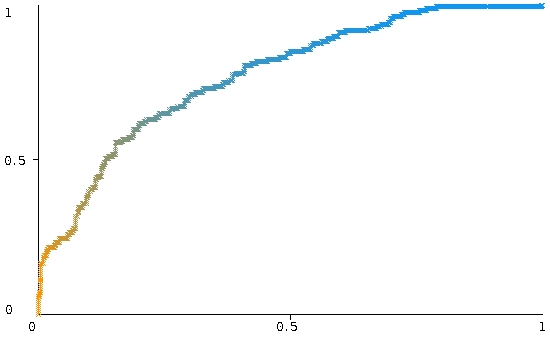
\includegraphics[width=\textwidth]{bayes_roc/roc_curve_b.jpg}
        \caption[]%
        {{\small The ROC for class B, the area under ROC is 0.7723.}}    
        \label{fig:bayes roc curve class b}
    \end{subfigure}
    \vskip\baselineskip
    \begin{subfigure}[b]{0.475\textwidth}   
        \centering 
        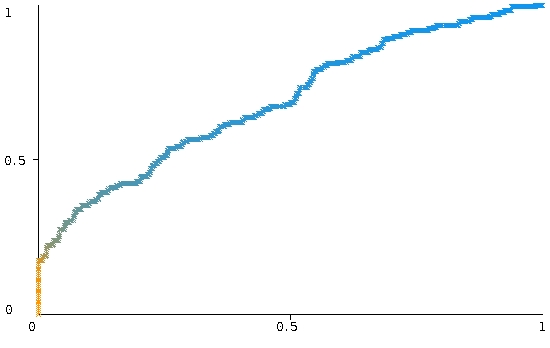
\includegraphics[width=\textwidth]{bayes_roc/roc_curve_c.jpg}
        \caption[]%
        {{\small The ROC for class C, the area under ROC is 0.6881.}}    
        \label{fig:bayes roc curve class c}
    \end{subfigure}
    \quad
    \begin{subfigure}[b]{0.475\textwidth}   
        \centering 
        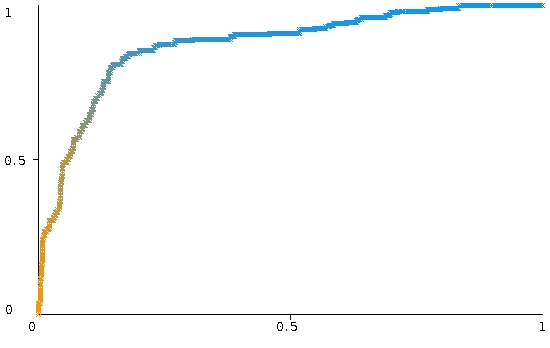
\includegraphics[width=\textwidth]{bayes_roc/roc_curve_e(d).jpg}
        \caption[]%
        {{\small The ROC for class E, the area under ROC is 0.8715.}}    
        \label{fig:bayes roc curve class d}
    \end{subfigure}
    \caption[The Receiver Operator Characteristic Curve for the Naive Bayes classifier]
    {\small The Receiver Operator Characteristic Curve for the Naive Bayes classifier} 
    \label{fig:naive bayes roc curves}
\end{figure*}

\begin{figure*}
    \centering
    \begin{subfigure}[b]{0.475\textwidth}
        \centering
        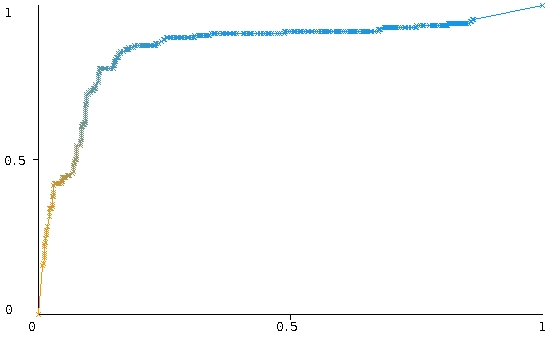
\includegraphics[width=\textwidth]{c45_roc/roc_curve_a.jpg}
        \caption[Network2]%
        {{\small The ROC for class A, the area under ROC is 0.8613.}}    
        \label{fig:c45 roc curve class a}
    \end{subfigure}
    \hfill
    \begin{subfigure}[b]{0.475\textwidth}  
        \centering 
        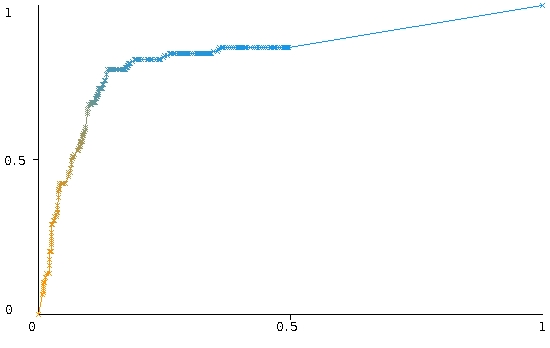
\includegraphics[width=\textwidth]{c45_roc/roc_curve_b.jpg}
        \caption[]%
        {{\small The ROC for class B, the area under ROC is 0.8341.}}    
        \label{fig:c45 roc curve class b}
    \end{subfigure}
    \vskip\baselineskip
    \begin{subfigure}[b]{0.475\textwidth}   
        \centering 
        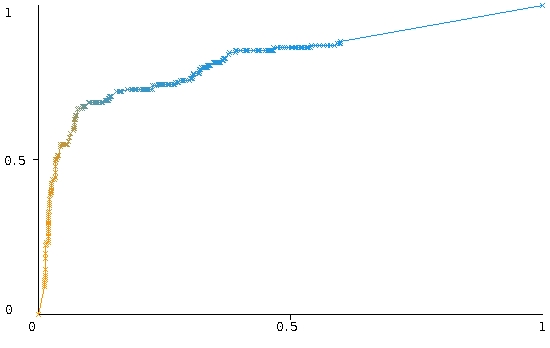
\includegraphics[width=\textwidth]{c45_roc/roc_curve_c.jpg}
        \caption[]%
        {{\small The ROC for class C, the area under ROC is 0.8208.}}    
        \label{fig:c45 roc curve class c}
    \end{subfigure}
    \quad
    \begin{subfigure}[b]{0.475\textwidth}   
        \centering 
        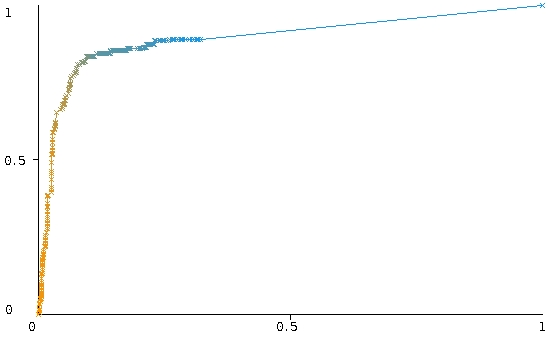
\includegraphics[width=\textwidth]{c45_roc/roc_curve_e(d).jpg}
        \caption[]%
        {{\small The ROC for class E, the area under ROC is 0.892.}}    
        \label{fig:c45 roc curve class d}
    \end{subfigure}
    \caption[The Receiver Operator Characteristic Curve for the J48 Classifier]
    {\small The Receiver Operator Characteristic Curve for the J48 Classifier} 
    \label{fig:c45 roc curves}
\end{figure*}

\subsection*{Part C}
 A baseline classifier provides a prediction in a very simple way, Weka includes a baseline classifier called ZeroR which works by predicting a majority class this achieved 29.25\% accuracy and since the two previous classifiers outperformed this they are better than the baseline. A baseline is important because it gives you a point of reference to allow you to compare other classifiers. If you couldn't get a result that was better than a baseline then it may mean that the problem you are trying to solve needs to be re-evaluated and solved in a different way.

\section*{Task 2}

\subsection*{Part A}
There are a few different ways of handling missing values. You could remove the missing values entirely so that data is no longer in the set or you could work out the average value for the missing data and use that. 

Replacing the missing values with the mean and mode sometimes isn't very meaningful because for binary features the mean could be somewhere in between the two values and you have to interpret that. You could improve upon this be using probability theory to look at the distributions and then take the missing value from that.

There is a filter in Weka called RepalceMissingValues, this replaces all missing values with the modes and means from the training data. When replacing missing values with the mean you could bias your dataset, to avoid this you should consider the mean and mode of all the instances from the training data rather than just from that class.

Another filter is the RemoveWithValues filter this allows you to filter and match certain pieces of data and then remove them, I used this to remove any data instance that had a missing attribute. 

If I were to replace values I would use the RepalceMissingValues filter.

\subsection*{Part B}
There are 46 missing values for the Reason\_for\_absence feature and 3 in the Month\_of\_absence feature, across all the instances and attributes there are only 49 missing values this amounts to 0.45\% of the total number of attributes so I don't think that there are enough missing values for it to make a difference if you replace these values. The missing values are all from the A absent class so if you do replace them then it might cause an increase in accuracy for that class.

\subsection*{Part C}

After replacing the missing values the overall accuracy for Naive Bayes was 57.75\% and the Kappa statistic was 0.4369. For J48 the overall accuracy was 74.003\% and the Kappa statistic was 0.652. The overall accuracy for both has gone up by about 2\% and the Kappa statistic has gone up by about 0.03 these both show the increase in performance that occurred after the missing values were replaced. The confusion matrices also show this increase in performance.

The J48 confusion matrix, figure \ref{fig:j48 changed confusion matrix}, shows the increase in performance for classes A, B and C The performance of E remains unchanged, this may be because there aren't any missing values that have an absent class of E.

The confusion matrix for Naive Bayes, figure \ref{fig:nb changed confusion matrix}, shows somewhat similar results with class A having the highest increase in accuracy, the value replacement had a negative impact on class B which may indicate that the values that have been replaced are wrong.

Table \ref{tab:valuetabletask2} shows the precision recall and F-Measure scores and when comparing these to the classifier before the value replacement you generally see an increase in performance, the low recall in C for Naive Bayes is still present. The performance for classifying B has fallen.

% Please add the following required packages to your document preamble:
% \usepackage{booktabs}
\begin{table}[]
\centering
\begin{tabular}{@{}|l|l|l|l|l|l|l|@{}}
\toprule
\begin{tabular}[c]{@{}l@{}}Absence\\  Class\end{tabular} & \begin{tabular}[c]{@{}l@{}}NB \\ Precision\end{tabular} & \begin{tabular}[c]{@{}l@{}}J48 \\ Precision\end{tabular} & \begin{tabular}[c]{@{}l@{}}NB \\ Recall\end{tabular} & \begin{tabular}[c]{@{}l@{}}J48 \\ Recall\end{tabular} & \begin{tabular}[c]{@{}l@{}}NB \\ F-Measure\end{tabular} & \begin{tabular}[c]{@{}l@{}}J48 \\ F-Measure\end{tabular} \\ \midrule
A                                                        & 0.498                                                   & 0.721                                                    & 0.671                                                & 0.730                                                 & 0.571                                                   & 0.725                                                    \\ \midrule
B                                                        & 0.455                                                   & 0.647                                                    & 0.579                                                & 0.704                                                 & 0.510                                                   & 0.675                                                    \\ \midrule
C                                                        & 0.667                                                   & 0.776                                                    & 0.298                                                & 0.661                                                 & 0.412                                                   & 0.714                                                    \\ \midrule
E                                                        & 0.754                                                   & 0.807                                                    & 0.742                                                & 0.843                                                 & 0.748                                                   & 0.825                                                    \\ \bottomrule
\end{tabular}
\caption{ A  table showing the Precision, Recall and F-Measure for Naive Bayes (NB) and J48 after replacing the missing values}
\label{tab:valuetabletask2}
\end{table}

%J48 confusion Matrix
\begin{figure*}
    \centering
    {
    \offinterlineskip
    \hspace*{1cm}\MyHBox{A}\MyHBox{B}\MyHBox{C}
    \MyHBox{E}\par
    
    \MyTBox{A}{111, 24, 8, 9}
    \MyTBox{B}{18, 112, 16, 13}
    \MyTBox{C}{15, 24, 111, 18}
    \MyTBox{E}{10, 13, 8, 167}
    }
    \caption{The confusion matrix for the J48 decision tree classifier after replacing the missing values.}
    \label{fig:j48 changed confusion matrix}
\end{figure*}

%NB confusion Matrix
\begin{figure*}
    \centering
    {
    \offinterlineskip
    \hspace*{1cm}\MyHBox{A}\MyHBox{B}\MyHBox{C}
    \MyHBox{E}\par
    
    \MyTBox{A}{102, 26, 10, 14}
    \MyTBox{B}{44, 92, 11, 12}
    \MyTBox{C}{37, 59, 50, 22}
    \MyTBox{E}{22, 25, 4, 147}
    }
    \caption{The confusion matrix for the Naive Bayes classifier after replacing the missing values.}
    \label{fig:nb changed confusion matrix}
\end{figure*}

\section*{Task 3}

\subsection*{Part A}

This newly trained classifier has performance that is relatively similar to the classifiers in Task 1 with J48 performing better than Naive Bayes and Naive Bayes performing particularly poorly on absence class C. The Precision, Recall and F-Measure values are shown in table \ref{tab:valuetabletask3}. This reduced dataset classifier generally performed worse, apart from the precision for Naive Bayes in class A and E, this will mean that the classifier has gotten better at predicting class A. The recall has also dropped so this demonstrates the precision recall trade off.

% Please add the following required packages to your document preamble:
% \usepackage{booktabs}
\begin{table}[]
\centering
\begin{tabular}{@{}|l|l|l|l|l|l|l|@{}}
\toprule
\begin{tabular}[c]{@{}l@{}}Absence\\  Class\end{tabular} & \begin{tabular}[c]{@{}l@{}}NB \\ Precision\end{tabular} & \begin{tabular}[c]{@{}l@{}}J48 \\ Precision\end{tabular} & \begin{tabular}[c]{@{}l@{}}NB \\ Recall\end{tabular} & \begin{tabular}[c]{@{}l@{}}J48 \\ Recall\end{tabular} & \begin{tabular}[c]{@{}l@{}}NB \\ F-Measure\end{tabular} & \begin{tabular}[c]{@{}l@{}}J48 \\ F-Measure\end{tabular} \\ \midrule
A                                                        & 0.473                                                   & 0.675                                                    & 0.461                                                & 0.684                                                 & 0.467                                                   & 0.680                                                    \\ \midrule
B                                                        & 0.406                                                   & 0.620                                                    & 0.667                                                & 0.648                                                 & 0.505                                                   & 0.634                                                    \\ \midrule
C                                                        & 0.580                                                   & 0.679                                                    & 0.238                                                & 0.631                                                 & 0.338                                                   & 0.654                                                    \\ \midrule
E                                                        & 0.729                                                   & 0.801                                                    & 0.732                                                & 0.813                                                 & 0.730                                                   & 0.807                                                    \\ \bottomrule
\end{tabular}
\caption{ A  table showing the Precision, Recall and F-Measure for Naive Bayes (NB) and J48 after removing some of the attributes}
\label{tab:valuetabletask3}
\end{table}

The new decision tree is of a smaller size than that in task 1 it has 87 leaves and a size of 148 whereas the tree from task 1 has 157 leaves and a total size of 213. This change in the tree size is because decision trees are non robust so a small change in the training data causes a large change in the tree\cite[p.316]{JamesGareth2013Aits}.

\subsection*{Part B}

I think that this classification problem is quite similar to that in task 1 because you are still trying to train a classifier to find out the absent class you are just doing this with a reduced data set. It is a harder problem because there is less data for the classifiers to work with this is why there is a decrease in accuracy. For a problem like this it does need quite a lot of attributes in the data because there are lots of factors in becoming absent from work and therefore differentiating these absences without all the data is not always possible. 

\bibliographystyle{plain}
\nocite{*}
\bibliography{bibliography.bib}

\begin{appendices}
\section{Receiver Operator Characteristic}
\label{appendix:roc}
This relates to Task 1 Part B.

A measure you could use is the Receiver Operator Characteristic Curve this is a plot of false positive rate along the x axis and true positive rate along the y axis, a perfect classifier would be a plot at (0,1) which would mean 100\% true positives and 0\% false positives. Figures \ref{fig:naive bayes roc curves} and \ref{fig:c45 roc curves} show these ROC curves and their Area Under Curve (AUC). The ROC curve is not useful in this context because it's not meant for multi class problems, in general it is useful for two class problems\cite{Hand2009} because the area under the curve represents how well the classifier differentiates between two classes. it is possible to create an ROC for multi class problems by changing the classification to be for one class and every other class, so for example how well it can classify class A and not class A. 


\end{appendices}

\end{document}  
%%%%%%%%%%%%%%%%%%%%%%%%%%%%%%%%%%%%%%%%%%%%%%